\documentclass[journal]{IEEEtran}
\usepackage{amsmath, amsfonts, graphicx, listings, xcolor, float, subfig}

\definecolor{codegreen}{rgb}{0,0.6,0}
\definecolor{codegray}{rgb}{0.5,0.5,0.5}
\definecolor{codepurple}{rgb}{0.58,0,0.82}
\definecolor{backcolour}{rgb}{0.95,0.95,0.92}

\lstdefinestyle{mystyle}{
    backgroundcolor=\color{backcolour},   
    commentstyle=\color{codegreen},
    keywordstyle=\color{magenta},
    numberstyle=\tiny\color{codegray},
    stringstyle=\color{codepurple},
    basicstyle=\ttfamily\footnotesize,
    breakatwhitespace=false,         
    breaklines=true,                 
    captionpos=b,                    
    keepspaces=true,                 
    numbers=left,                    
    numbersep=5pt,                  
    showspaces=false,                
    showstringspaces=false,
    showtabs=false,                  
    tabsize=2
}

\lstset{style=mystyle}

\graphicspath{ {./images/} } % tells LaTeX that the images are kept in a folder named images under the directory of the main document.

\title{Lab 2: Statistical Functions and plot Histograms}
\author{
    \IEEEauthorblockN{Argenis Aquino, Rachel DuBois, Diego Lopez, Jonathan Sumner \\}
    \IEEEauthorblockA{
        Department of Engineering Technology, Rochester Institute of Technology\\
        1 Lomb Memorial Drive, Rochester NY, 14623, United States of America \\
    }
}

\begin{document}
\maketitle

\begin{abstract}
    This document shows how MATLAB was used to gain experience using the statistical functions provided to process digital signals. Participants analyzed data using MATLAB commands to find data such as a samples max, mean, and standard deviation as well as explored the use of the histogram function to estimate and characterize the probability density function of random variables.
\end{abstract}

\section{Introduction}
\IEEEPARstart{M}{ATLAB} gives users access to statistical functions that can be used to process data in various ways. Here methods such as std were used in order to find values that would help important information such as the signal to noise ratio (SNR). Plots were used to visualize the difference between quantized and quantized error signals.

\section{Methodology}
The procedure started with loading given data from a .mat file into the MatLab workspace. With the give data the max, minimum, and mean values were found along with the standard deviation and variance.
\begin{lstlisting}[language=matlab]
    clear
    load Lab2_Chapter2_Section1.mat
    [sample, signal]
    
    maxSignal = max(signal)
    minSignal = min(signal)
    avgSignal = mean(signal)
    stdSignal = std(signal)
    varSignal = var(signal)
\end{lstlisting}

The values loaded from the .mat file were used to create a plot and histogram.
\begin{lstlisting}[language=matlab]
    figure
    plot(sample, signal, 'LineWidth', 1)

    %  Solution -- Place your code to label the axes and title the graph

    grid on % Display or hide axes grid lines
    hold on % Retain current plot when adding new plots

    title('Signal versus Sample') % Custom title

    % Axis labels
    xlabel('Signal')
    ylabel('Sample')

    legend('Signal') % Legend to show which lines are which
    hold off

    histogram(signal)
    grid on
    
    title('Signal Histogram') % Custom title
    
    % Axis labels
    xlabel('Signal')
    ylabel('Frequency')
\end{lstlisting}

\section{Results}

\begin{figure}[h] % Fig 1
    \centering
    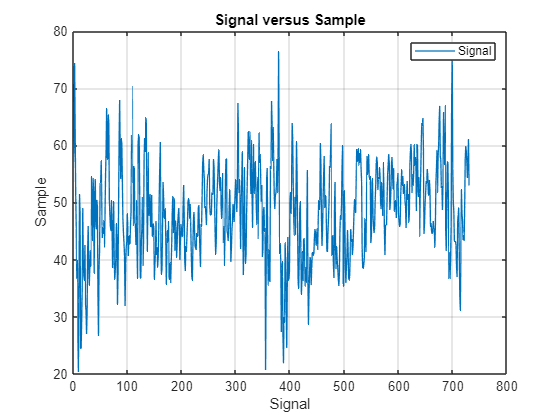
\includegraphics[width=\linewidth]{1.3.png}
    \caption{Original Signal}
    \vspace{1em} % Adds vertical space
    \begin{minipage}{\linewidth}
        \small
        In Figure 1, the original signal is plotted against the samples. This plot allows the max and minimum sample number to be estimated by observing the figure.
    \end{minipage}
    \label{Part 1.1: Signal vs Sample plot}
\end{figure}

\begin{figure}[ht] % Fig 2
    \centering
    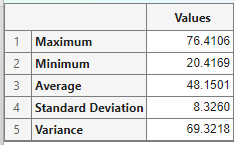
\includegraphics[width=\linewidth]{1.2.png}
    \caption{Table with the estimated values}
    \vspace{1em} % Adds vertical space
    \begin{minipage}{\linewidth}
        \small The values from the max, min, mean, std, and var functions were inserted into this table. These values were used to compare the accuracy against the histogram with teh actualy values.
    \end{minipage}
    \label{Part 1: Estimated Value Table}
\end{figure}

\begin{figure}[ht] % Fig 3
    \centering
    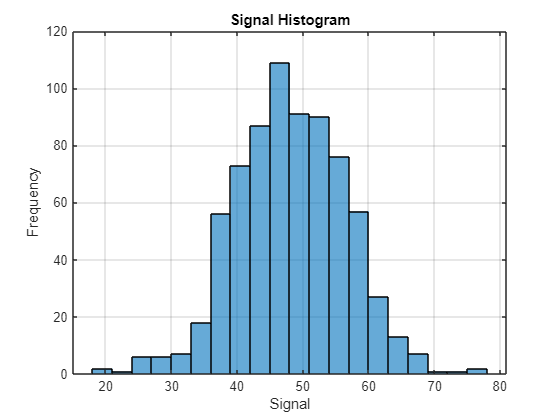
\includegraphics[width=\linewidth]{1.5.png}
    \caption{Histogram of the actual values}
    \vspace{1em} % Adds vertical space
    \begin{minipage}{\linewidth}
        \small This figure shows a histogram with the actual statistical values. With this graph we can  
    \end{minipage}
    \label{Part 1: Signal vs Frequency Histogram}
\end{figure}

\section{Analysis}
Matlab makes me wanna jump infront of a moving car.

\section{Conclusion}

\end{document}